
\chapter{Surface Imaging}

\section{Introduction}

Atomic force microscopy (AFM) is a powerful tool for surface imaging, providing high-resolution topographical maps of sample surfaces. This technique is pivotal for understanding the morphology and texture of materials at the nanoscale. In this study, AFM was employed at various stages to quantitatively analyze the surface roughness of different materials.

\begin{figure}[h!!!!!!!]     %Insert a figure as soon as possible
        \begin{center}
          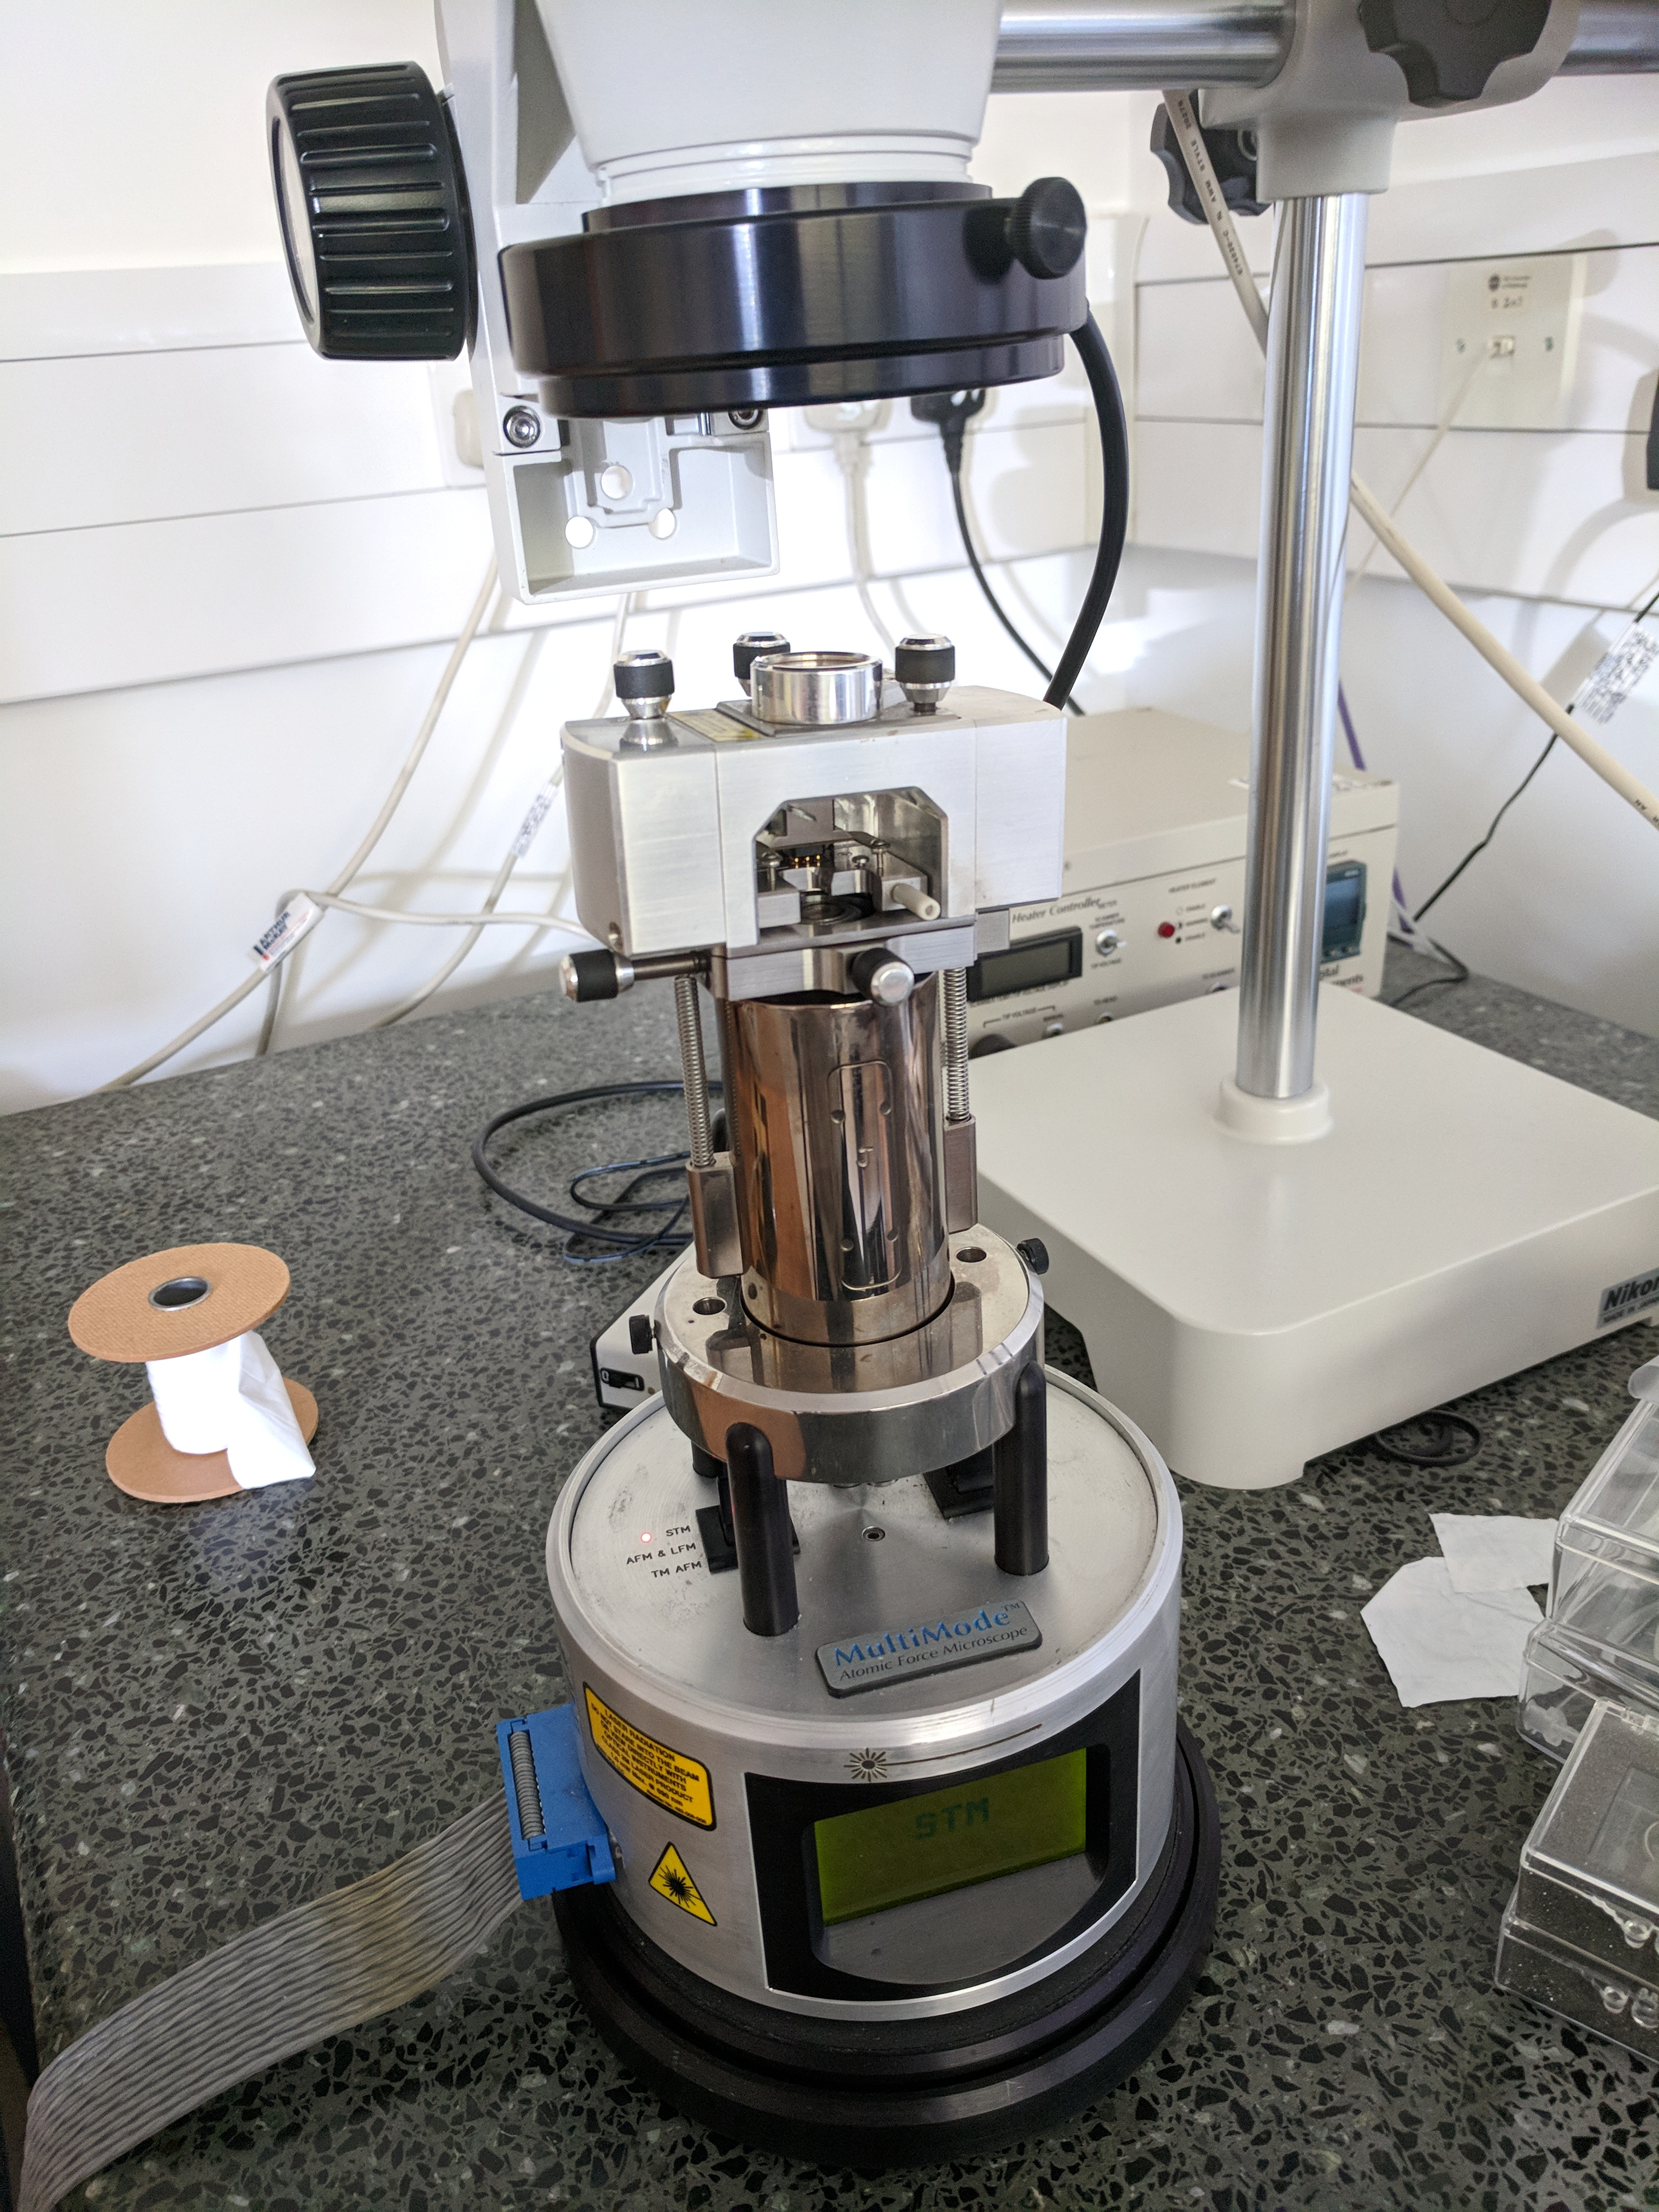
\includegraphics[width=70mm]{chapter2/ImageAFM.jpg}
\end{center}
\caption{Photograph of the operational setup for the Bruker Nanoscope 2, which was used for image measurements.}
\label{fig:ImageAFM}                 % Reference label to the figure.
\end{figure}

For the imaging purposes, we utilized the Bruker Nanoscope 2 AFM system shown in \ref{fig:ImageAFM}. This system is designed with a sample stage capable of securing a 1cm disc, integrated with the J scanner piezoelectric stage for precise movement. The optical alignment of the laser onto the cantilever is achieved using a finely adjustable mirror mechanism, with the head unit being stabilized by tension springs to ensure accurate tracking of surface contours.

\section{Surface analysis}

\subsection{Measuring the surface of mica}

In order to assess the capabilities of the AFM a freshly cleaved mica surface was scanned under the AFM. As mica is assumed to be atomically flat \cite{MicaSurf, Ostendorf_2008}. The cleavage of mica along its basal plane typically results in a smooth and featureless topography, making it an ideal substrate for AFM calibration and analysis.

\begin{figure}[h!!!!!!!]     %Insert a figure as soon as possible
        \begin{center}
          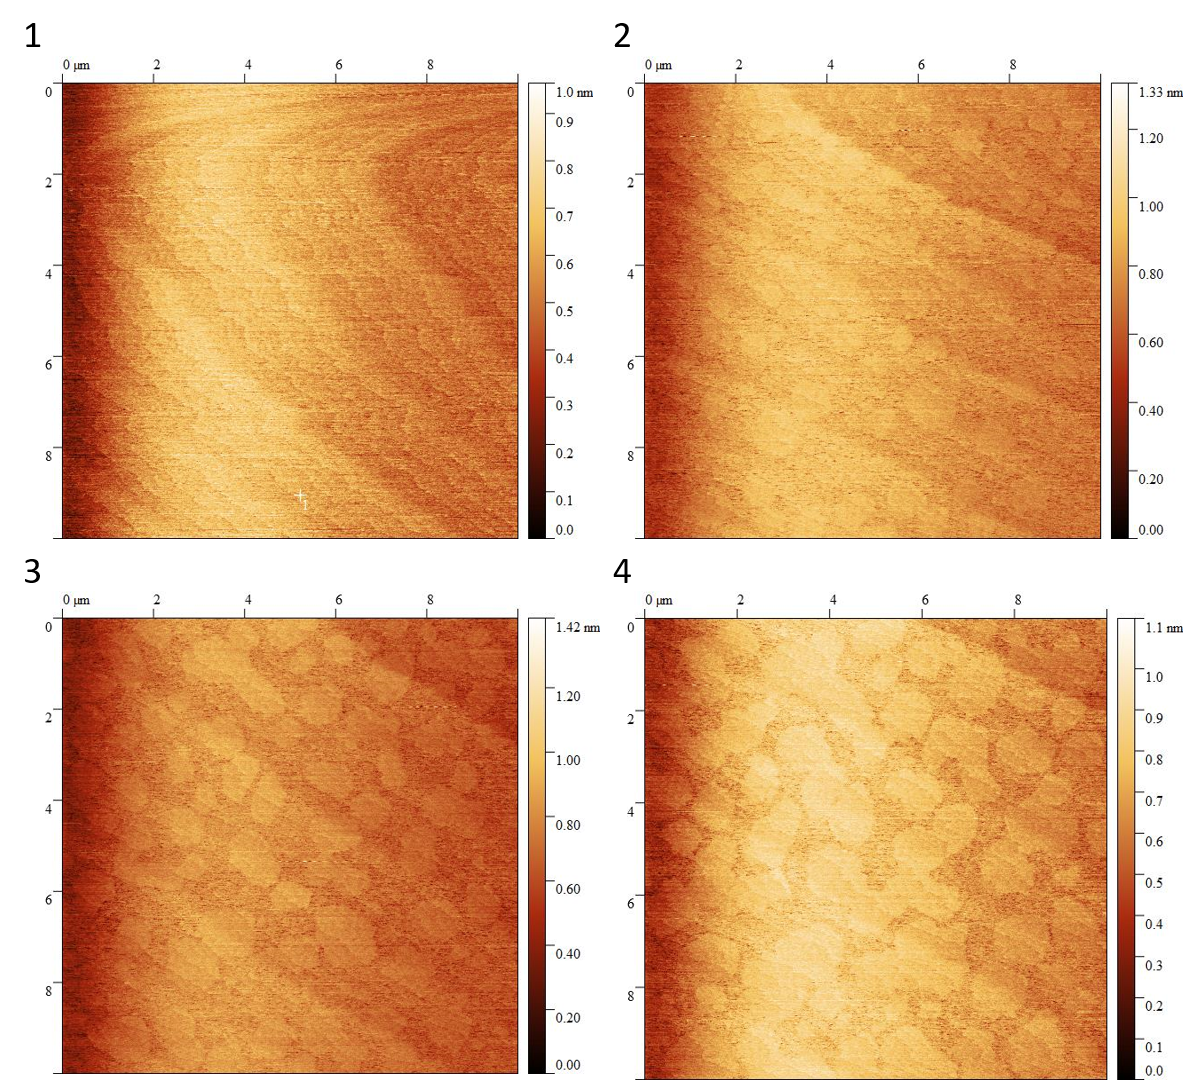
\includegraphics[width=110mm]{chapter3/Mica hydration.png}
\end{center}
\caption{Time-lapse AFM tapping mode images of a mica surface showing progressive hydration. The first image was taken roughly 10 minutes after cleavage, with each subsequent image taking about 30 minutes to take. The changes in surface texture and color intensity suggest the absorption of water from the air, leading to a more pronounced hydration pattern, as seen in the increased contrast and the development of distinct features over time.}
\label{fig:ImageAFM2}                 % Reference label to the figure.
\end{figure}

When a mica surface is freshly cleaved and exposed to air, it is expected to present an initially smooth and flat surface at the atomic level due to its layered crystalline structure, which allows for easy cleavage along the basal plane. However, when exposed to ambient air, the mica surface can begin to adsorb water molecules due to its hygroscopic nature, leading to the formation of a hydration layer from the hydration process. This process is gradual and can be observed as an increasing surface roughness or the development of hydration-related features in AFM images over time. \cite{MicaSurf, MicaHgryo, Koishi2022WaterAdsorption}

\subsection{Silica Surface Analysis}

 One common sample that was regularly imaged across the entire investigation was silica, be it a silica sphere or borosilica glass surface. A range of different types of silica surfaces was investigated as well as surface treatment techniques performed on the same glass surface. Initially borosilicate glass capillaries were investigated. This investigation intended to resolve the uniformity of a borosilicate capillary across multiple capillaries by profiling the surface topology and roughness across a range of different points. This glass capillary was then cross referenced against the petri dish in use, to ensure that the surface of the petri dish was representative of borosilicate glass. This surface was then referenced against scanning electron microscopy images of the tips, alongside inverted AFM imaging of the tip. 

Initially the inside of a glass capillary was imaged. The inside of the capillary was imaged by scoring the glass with a diamond tipped pen, with pressure applied on the outside to break the glass cleanly open \ref{fig:figure8}. This glass reference was used as a representation for the borosilica glass roughness used in Chapter 4 and 8, as the petri dish used in chapter 4 was too large to fit into the AFM. This borosilicate capillary was used due to the ability to modify the geometry into a suitable shape to fit into the imaging AFM available. As the imaging AFM is head mounted, the ability to image larger objects was not possible as this solution was reached due to availability of said capillaries.

\begin{figure}[h]     %Insert a figure as soon as possible
        \begin{center}
          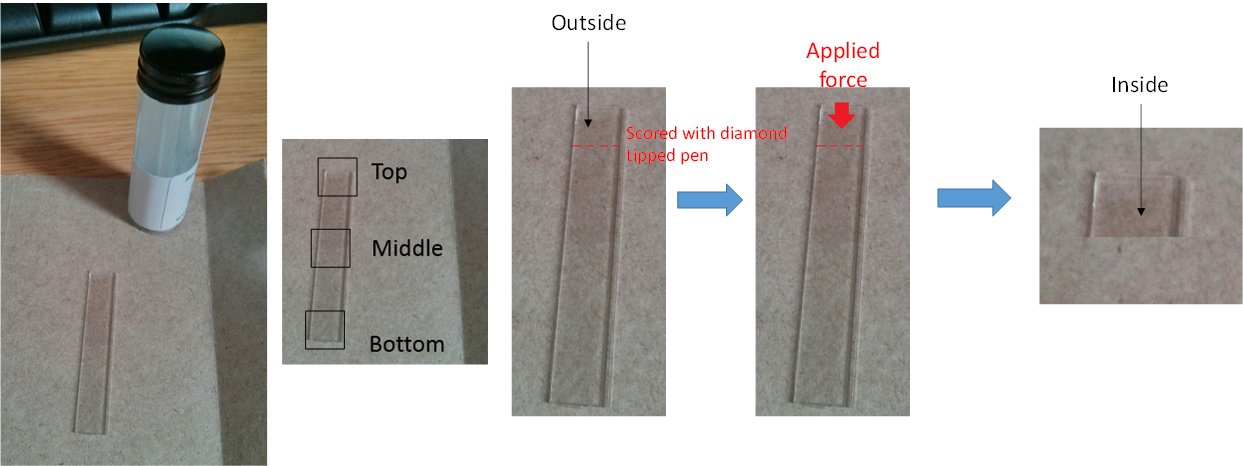
\includegraphics[width=120mm]{chapter3/Figure8.png}
\end{center}
\caption{A diagram demonstrating how the glass capillary was broken and how samples were extracted from the capillary.}
\label{fig:figure8}                 % Reference label to the figure.
\end{figure}   


The sample was then loaded inside up into the AFM under tapping mode operation in air. Multiple antimony doped silicon tips (Bruker RFESP-40 tips) were used to scan several samples each, giving a range of tips used for imaging. This was done to reduce any tip artifacts or degradation of tips so that image quality was retained throughout. A constant scan rate of 0.4Hz across all samples with the integral and proportional gain determined using the initial sample, then kept constant at 0.22 and 0.63 respectively. This was done to produce images that were similar as possible to one another from a parameter point of view. Large hysteresis effects present in the pizeo was negated by a small dummy scan window, where the AFM was left to run for a few seconds then reset to the origin of the scan. Each capillary was imaged 12 times at a 10 $\mu$m x 10 $\mu$m scan size followed by a 2 $\mu$m x 2 $\mu$m scan size. Images were taken at the top, the middle and the bottom of the capillary with a repeat image taken per site. Finally, two capillaries were imaged giving a total of 24 images. Scan sizes were chosen to give a larger view of the surface, while also scanning an area similar in size to the cantilever head used during the preliminary exploratory experiments (1.6 $\mu$m x 1.6 $\mu$m). The bead size was later increased to 6.6 $\mu$m during the course of the exploration, representing the final dataset (see chapter 4). 

In the case where dust was present in the images, to allow the applicability of a wider dataset, a standard method was used to handle dust. This involved two steps: image processing and visual inspection. After mean plane subtraction to correct for image tilt and alignment using a 5th order polynomial transformation, the images are closely examined. Dust is recognized by its consistency across all open-air images. To isolate and remove dust from the analysis, the z-axis range is adjusted, effectively minimizing the prominence of the dust in the visual representation. This method enhances the clarity of the underlying surface topology in the resultant images. Dust was only present in a small selection of the images.

\begin{figure}[h]     %Insert a figure as soon as possible
        \begin{center}
          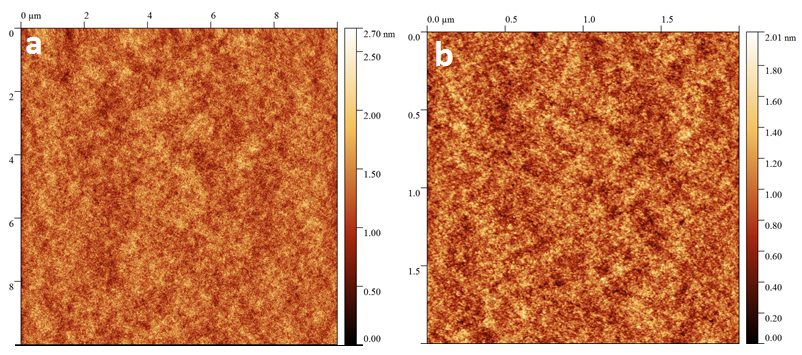
\includegraphics[width=120mm]{chapter3/Figure9.png}
\end{center}
\caption{Two sample AFM images of untreated borosilicate glass at two different scan sizes: (a) displays an image with a scan size of 10 $\mu$m x 10 $\mu$m, while (b) demonstrates a scan size of 2 $\mu$m x 2 $\mu$m.}
\label{fig:figure9}                 % Reference label to the figure.
\end{figure}   

\newpage
\subsubsection{Results}

The images for the inside top part of the capillary shown in \ref{fig:figure8} are shown below:

\begin{figure}[h!!!!]     %Insert a figure as soon as possible
        \begin{center}
          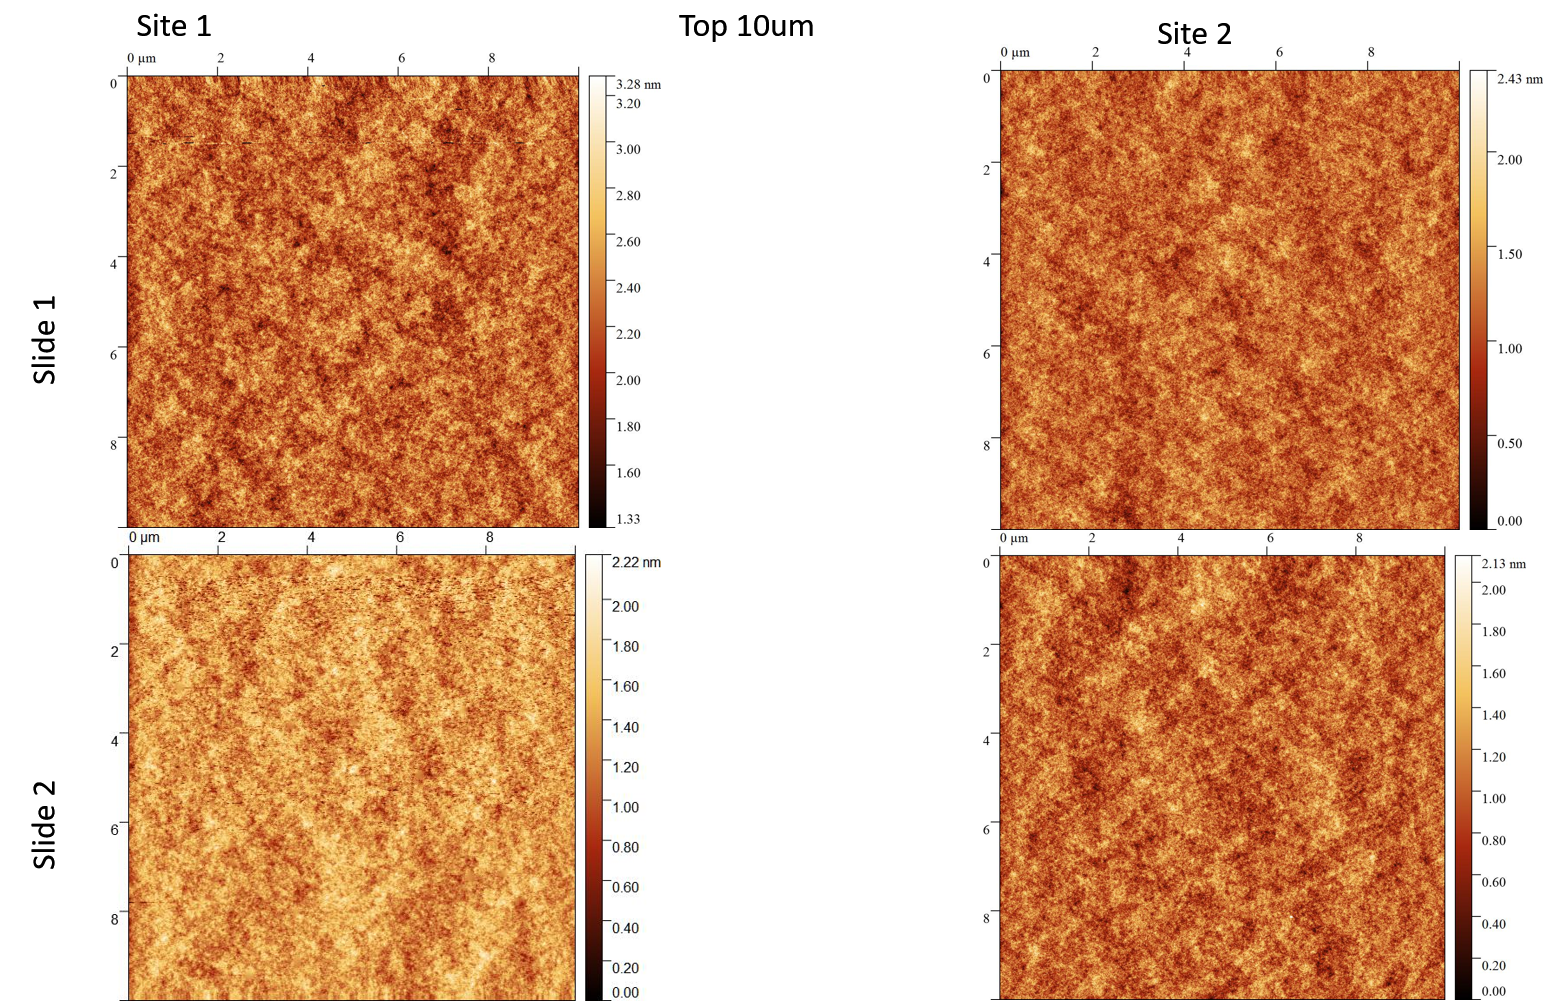
\includegraphics[width=100mm]{chapter3/Top 10um.png}
\end{center}
\caption{Four AFM images of untreated borosilicate glass on two different glass surfaces, with two sites per glass slide. The image has a scan size of 10 $\mu$m x 10 $\mu$m.}
\label{fig:figure9}                 % Reference label to the figure.
\end{figure}   

\begin{figure}[h!!!!]     %Insert a figure as soon as possible
        \begin{center}
          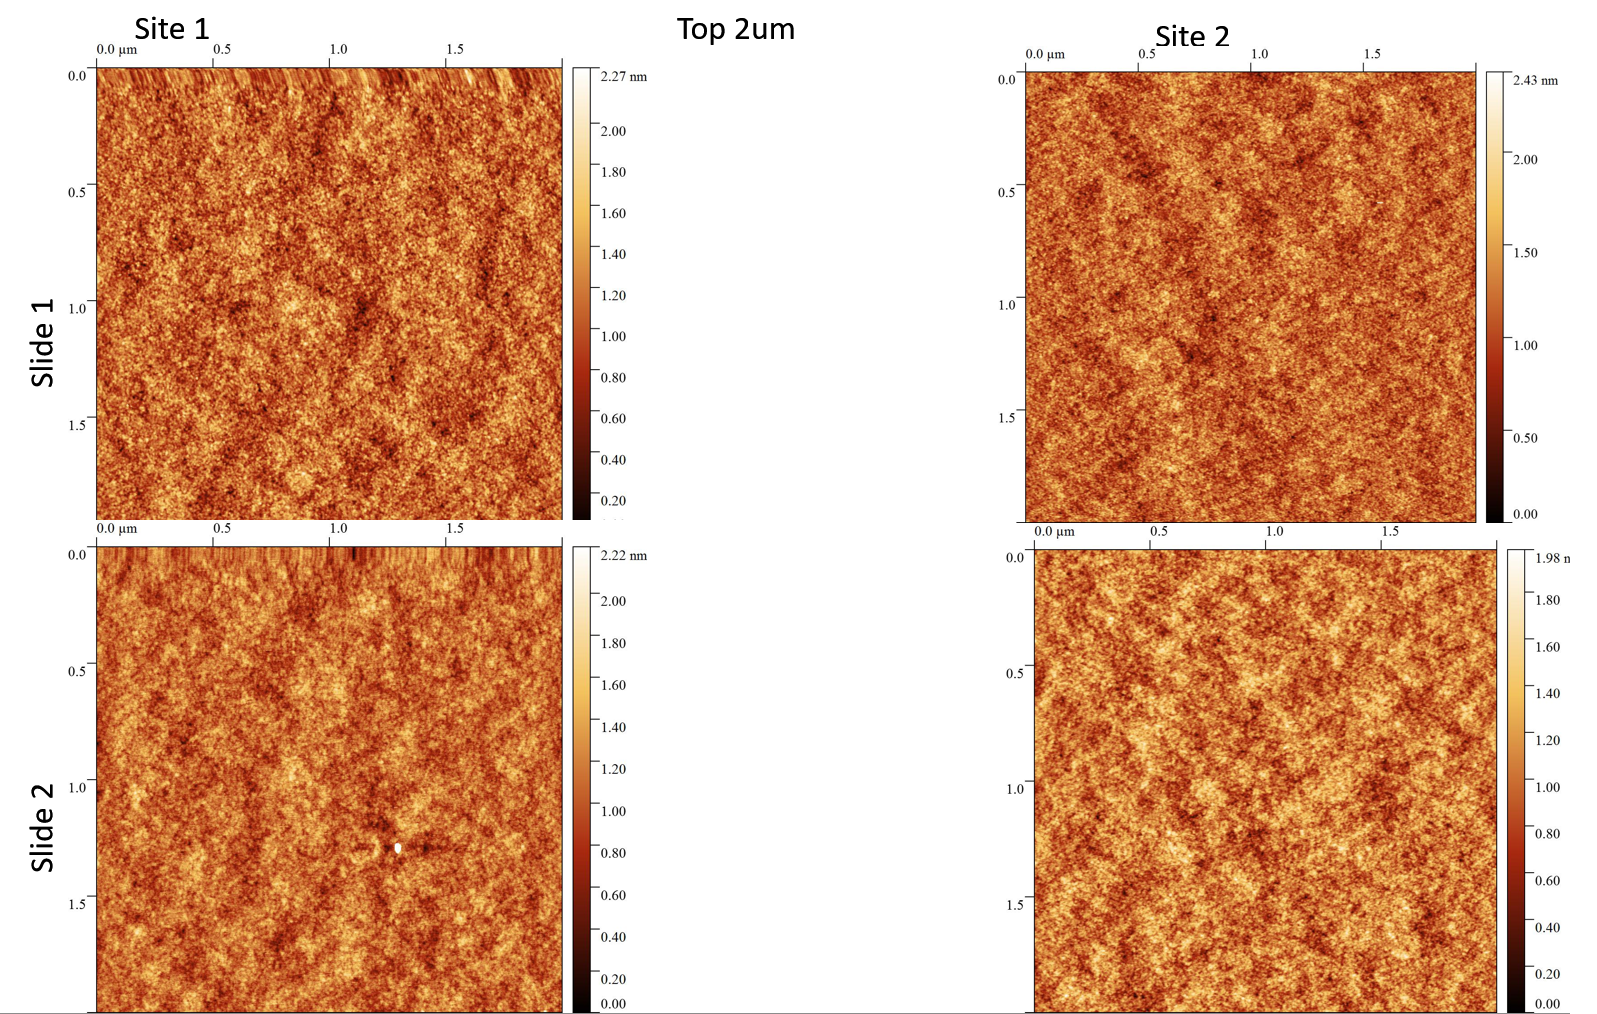
\includegraphics[width=100mm]{chapter3/Top 2um.png}
\end{center}
\caption{Four AFM images of untreated borosilicate glass on two different glass surfaces, with two sites per glass slide. The image has a scan size of 2 $\mu$m x 2 $\mu$m.}
\label{fig:figure9}                 % Reference label to the figure.
\end{figure}   

\newpage
The images for the inside middle part of the capillary shown in \ref{fig:figure8} are shown below:

\begin{figure}[h!!!!]     %Insert a figure as soon as possible
        \begin{center}
          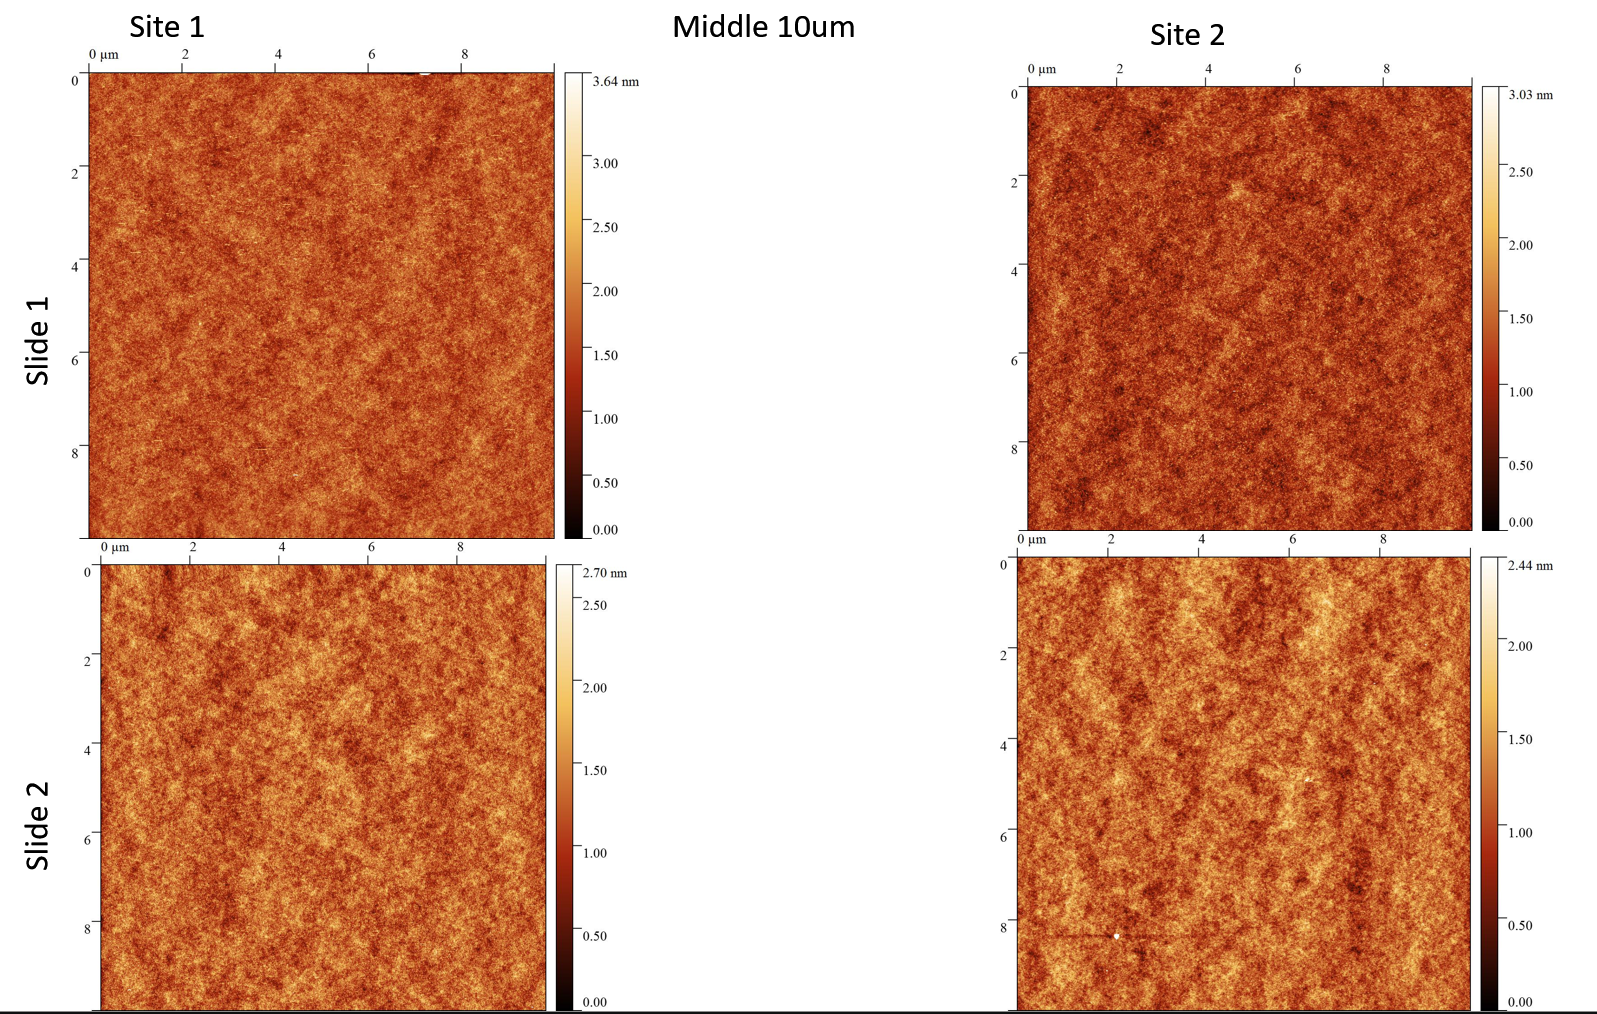
\includegraphics[width=100mm]{chapter3/mid 10um.png}
\end{center}
\caption{Four AFM images of untreated borosilicate glass on two different glass surfaces, with two sites per glass slide. The image has a scan size of 10 $\mu$m x 10 $\mu$m.}
\label{fig:figure9}                 % Reference label to the figure.
\end{figure}   

\begin{figure}[h!!!!]     %Insert a figure as soon as possible
        \begin{center}
          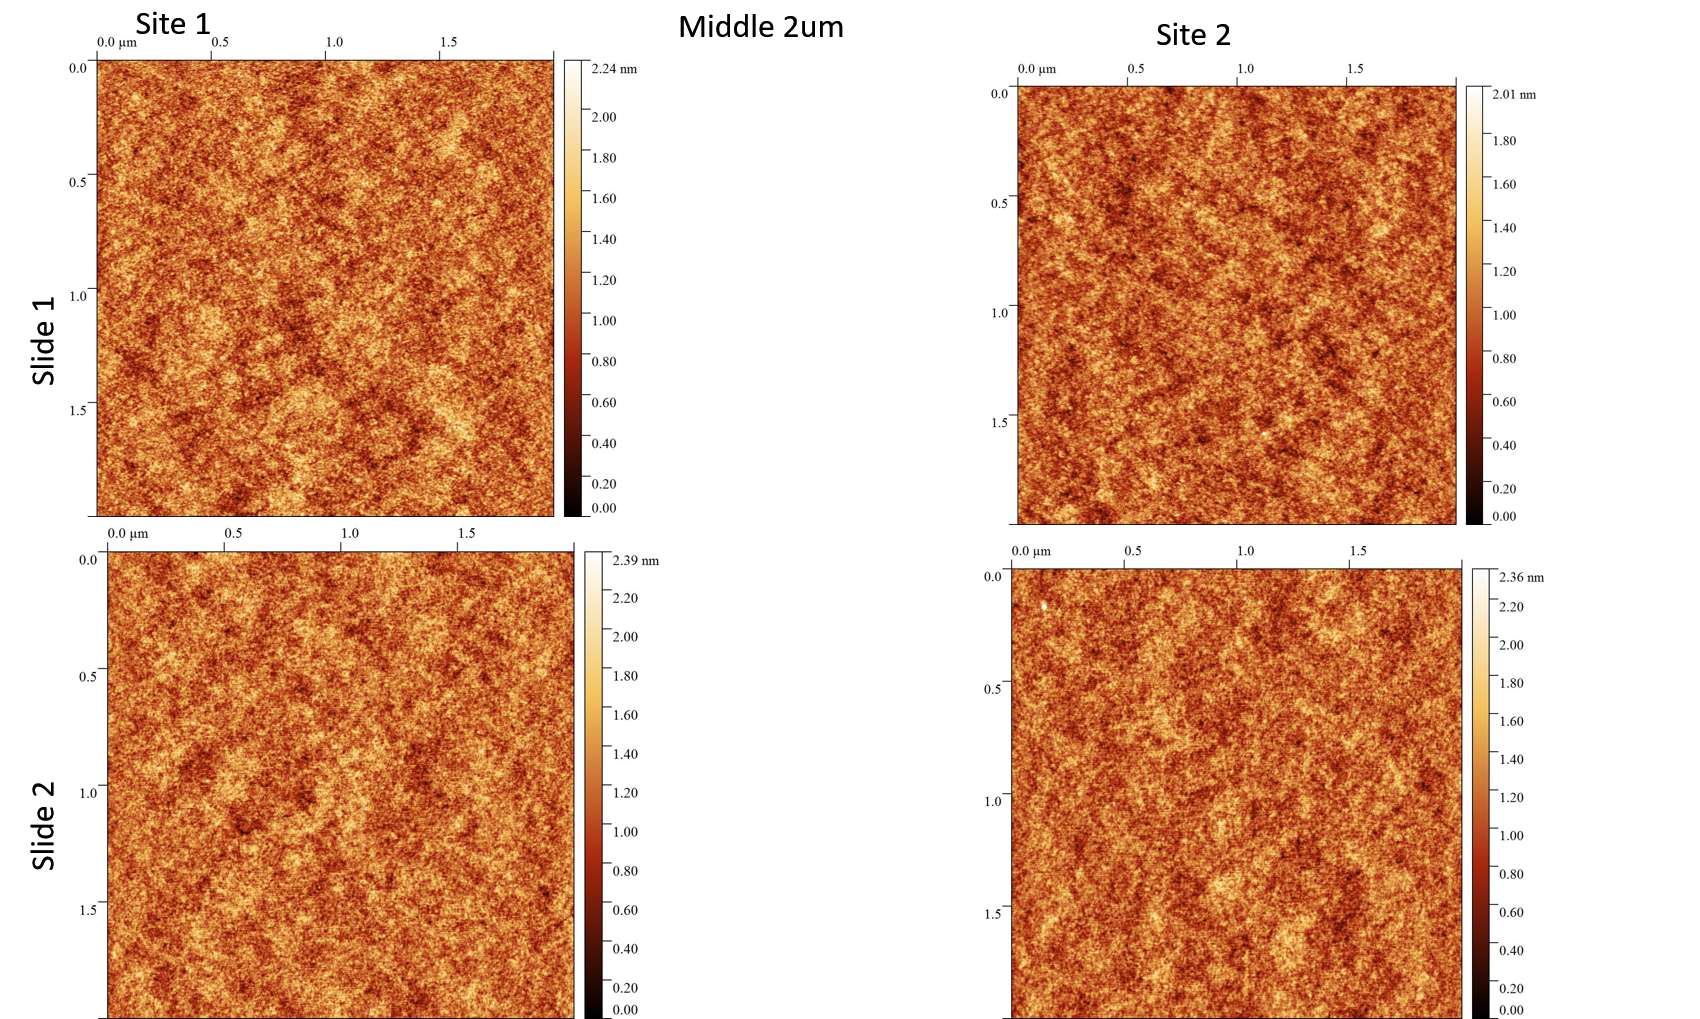
\includegraphics[width=100mm]{chapter3/mid 2um.png}
\end{center}
\caption{Four AFM images of untreated borosilicate glass on two different glass surfaces, with two sites per glass slide. The image has a scan size of 2 $\mu$m x 2 $\mu$m.}
\label{fig:figure9}                 % Reference label to the figure.
\end{figure}   

\newpage
The images for the inside bottom part of the capillary shown in \ref{fig:figure8} are shown below:

\begin{figure}[h!!!!]     %Insert a figure as soon as possible
        \begin{center}
          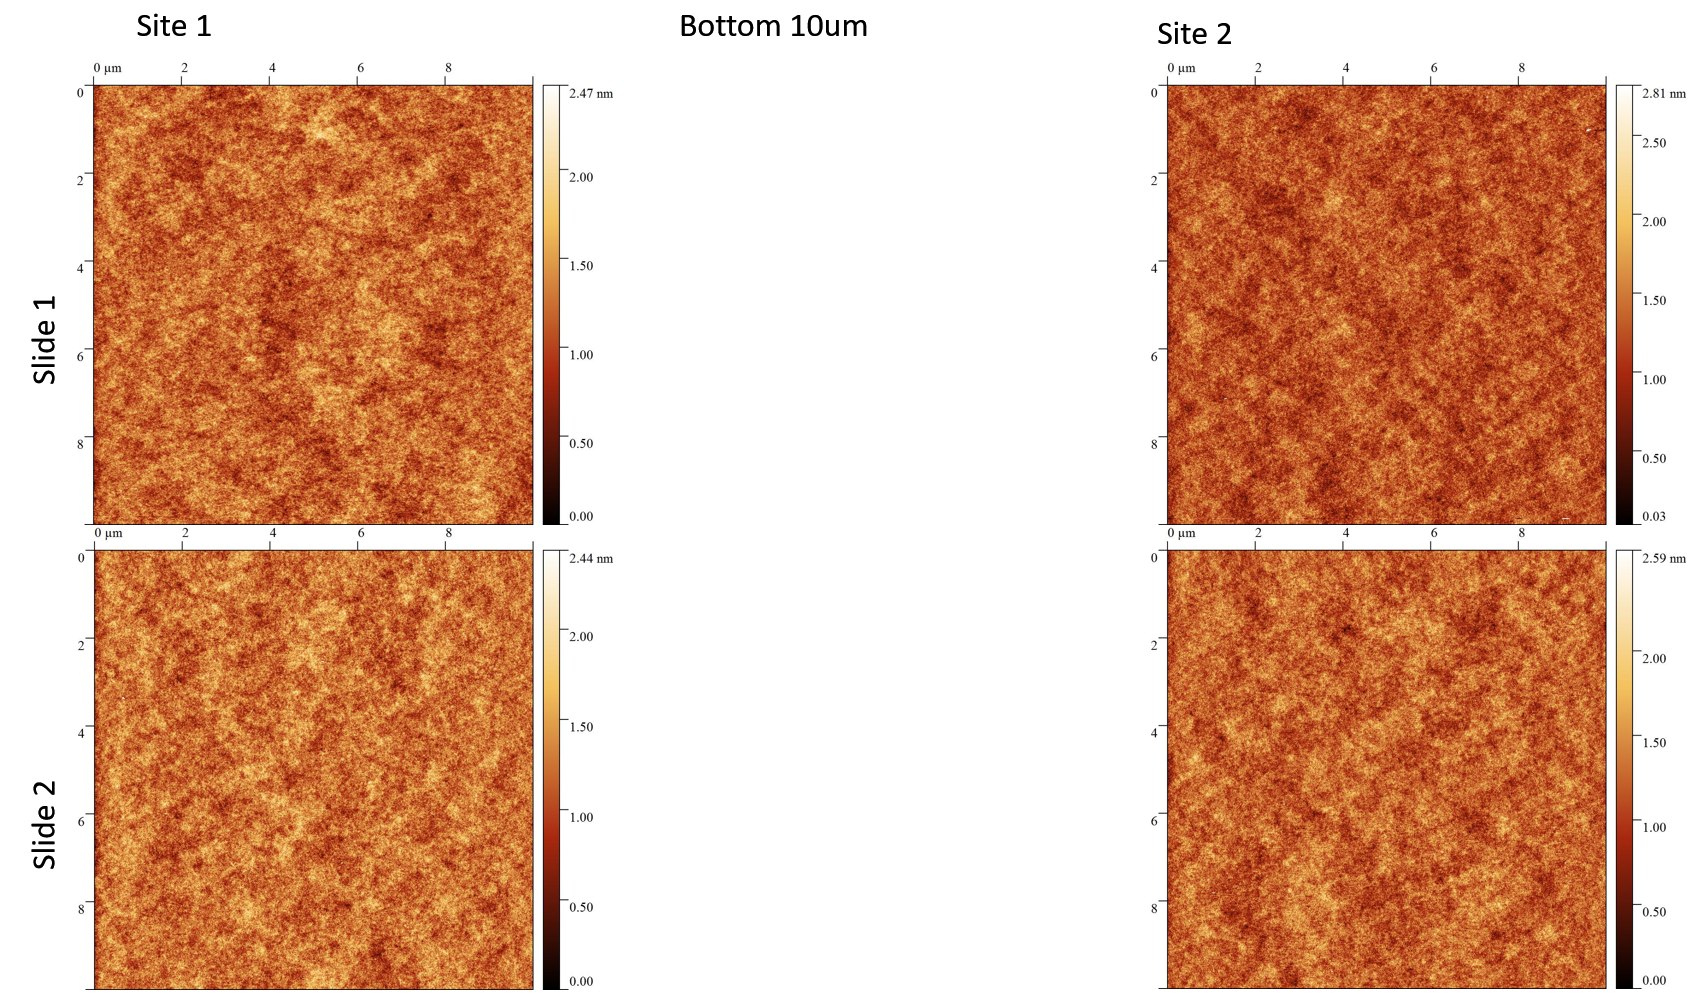
\includegraphics[width=100mm]{chapter3/bot 10um.png}
\end{center}
\caption{Four AFM images of untreated borosilicate glass on two different glass surfaces, with two sites per glass slide. The image has a scan size of 10 $\mu$m x 10 $\mu$m.}
\label{fig:figure9}                 % Reference label to the figure.
\end{figure}   

\begin{figure}[h!!!!]     %Insert a figure as soon as possible
        \begin{center}
          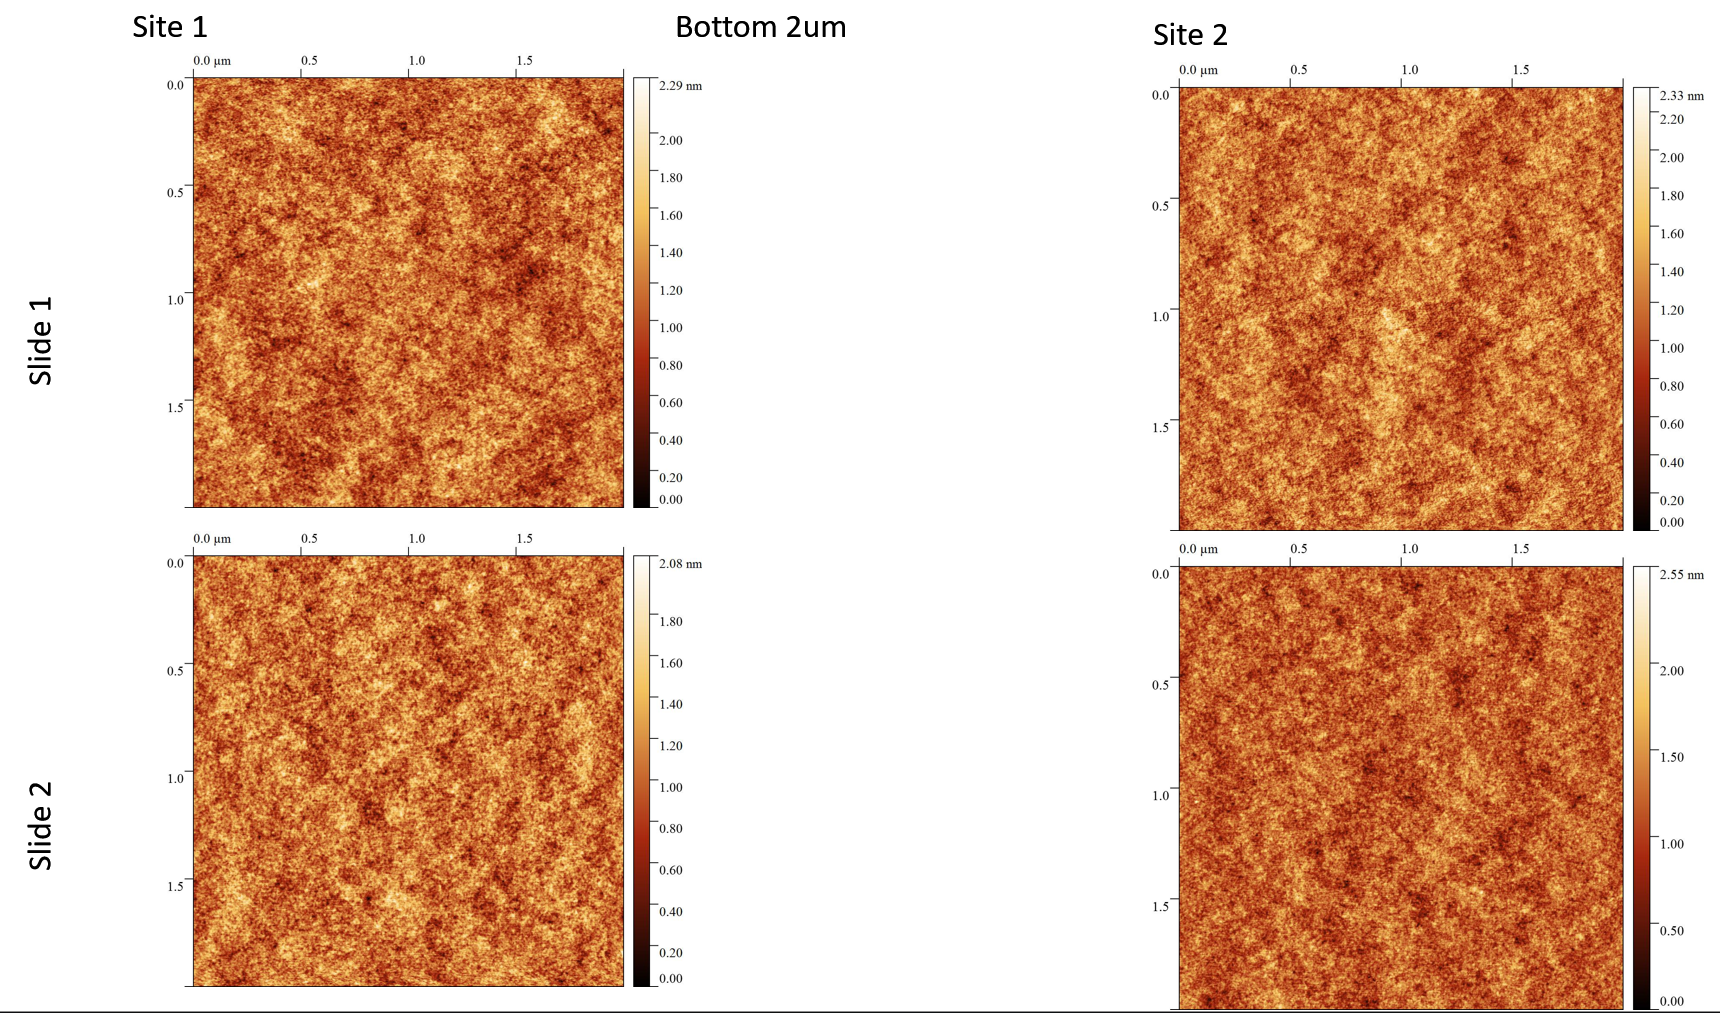
\includegraphics[width=100mm]{chapter3/bot 2um.png}
\end{center}
\caption{Four AFM images of untreated borosilicate glass on two different glass surfaces, with two sites per glass slide. The image has a scan size of 2 $\mu$m x 2 $\mu$m.}
\label{fig:figure9}                 % Reference label to the figure.
\end{figure}   

Gwyddion, an AFM analysis software, was used to process the resulting data from the imaging process and produce the images given in the figures above.\cite{gwy}

The AFM analysis of borosilicate glass surfaces demonstrated remarkable uniformity across the dataset of 24 images. The root mean square (RMS) roughness is a statistical measure of surface texture, calculated from the height data obtained in AFM imaging. RMS roughness is determined by taking the square root of the average of the squares of the height deviations from the mean plane of the surface within the scanned area. This gives a quantitative assessment of the surface's vertical irregularities. Additionally, peak-to-peak roughness in Gwyddion refers to the difference in height between the highest and lowest points within the scanned area, providing a direct measure of the surface's vertical variation.

Notably, the maximum peak-to-peak roughness average across the 24 image dataset was measured at 3.6 nm for images with a scan size of 10 $\mu$m x 10 $\mu$m, and 2.6 nm for those at 2 $\mu$m x 2 $\mu$m. The average root mean square (RMS) roughness values, calculated from the height variations across the scanned area, were 0.24 nm +/- 0.01 nm for 10 $\mu$m x 10 $\mu$m images and 0.2 nm +/- 0.02 nm for 2 $\mu$m x 2 $\mu$m images. These RMS values reflect the average height deviations from the mean plane with the standard deviation, providing a quantifiable measure of surface texture. Together the RMS was 0.2 nm +/- 0.02 nm. The consistency of the RMS roughness across both image sizes and sites indicates a homogenous surface texture irrespective of the scan area. Figure \ref{fig:figure9} presents representative images from each scan size category, illustrating the general surface topology observed. The consistent topology and roughness throughout the capillary's length and across multiple capillaries suggest that the surfaces used in the main investigation bear a similar structure to those depicted in Figure \ref{fig:figure9}.\cite{AFMbactPaper}
  

\subsubsection{Drift anaylsis}

In order to ensure that any error incurred by physical drift was accounted for an investigation into the x, y and z axis drift was explored. The AFM was left to image the same glass sample repeatedly in order to produce the same image several times. This image was then two dimensionally cross correlated with the next image in the sequence and the difference removed between the two z data points. The results are displayed in Figure\ref{fig:CrossCor}.

\begin{figure}[h]     %Insert a figure as soon as possible
        \begin{center}
          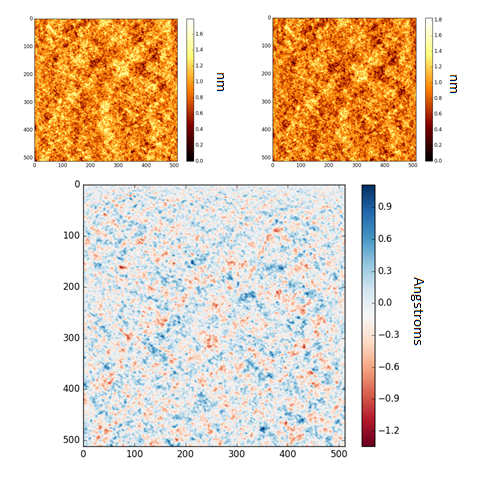
\includegraphics[width=120mm]{chapter3/CrossCor.png}
\end{center}
\caption{The output image of the 2D cross correlation function between the two images. The two smaller images are the input images into the script. The x and y values are the location of the z values in the 2D matrix dataset. The z scale is labeled respectively.}
\label{fig:CrossCor}                 % Reference label to the figure.
\end{figure}

Due to the drift experienced while scanning, the rows were found to be increasingly misaligned towards the bottom of the image. The result of this is shown by the gradient seen from the top of the image downwards , as the first image scanned from the bottom up, then the second image was scanned from the top down. The process was repeated on a row by row alignment basis and the resultant drift between the two images was found to be approximately 1 \AA{}ngstrom on the z axis, 8 nm on the y axis and 28 on the x axis. However given the speed of the scan was low at 0.4 Hz each image took approximately 40 minutes to image, giving an approximate drift of 0.1 nm by 0.5 nm drift per minute.

It was concluded from this analysis that the artificial effects of drift on the measured surface roughness would ultimately be negligible. Due to the small drift observed over time the influence of the resulting plane angle at points drifted towards would not have a large enough influence to impact the calculated roughness.

%Surface treatment



%\section{Glass surface cleaning}

%In order to ensure that the glass used in experiments was free of contaminants a study was performed to determine the cleanliness of the surface.



%SILICA TIP SURFACE

\section{Silica particle surface resolution} % MOVE TO CHAPTER 3 PLEASE

In order to determine the surface roughness of a silica sphere, a range of 1.5 $\mu m$ silica spheres were placed upon a suitable surface and imaged. The objective was to discern any roughness variances between a flat silica surface and a spherical one. The methodology was influenced by the AFM tips used in in Chapter 4, which involved cantilevers with silica spheres attached.



\begin{figure}[h]     %Insert a figure as soon as possible
        \begin{center}
          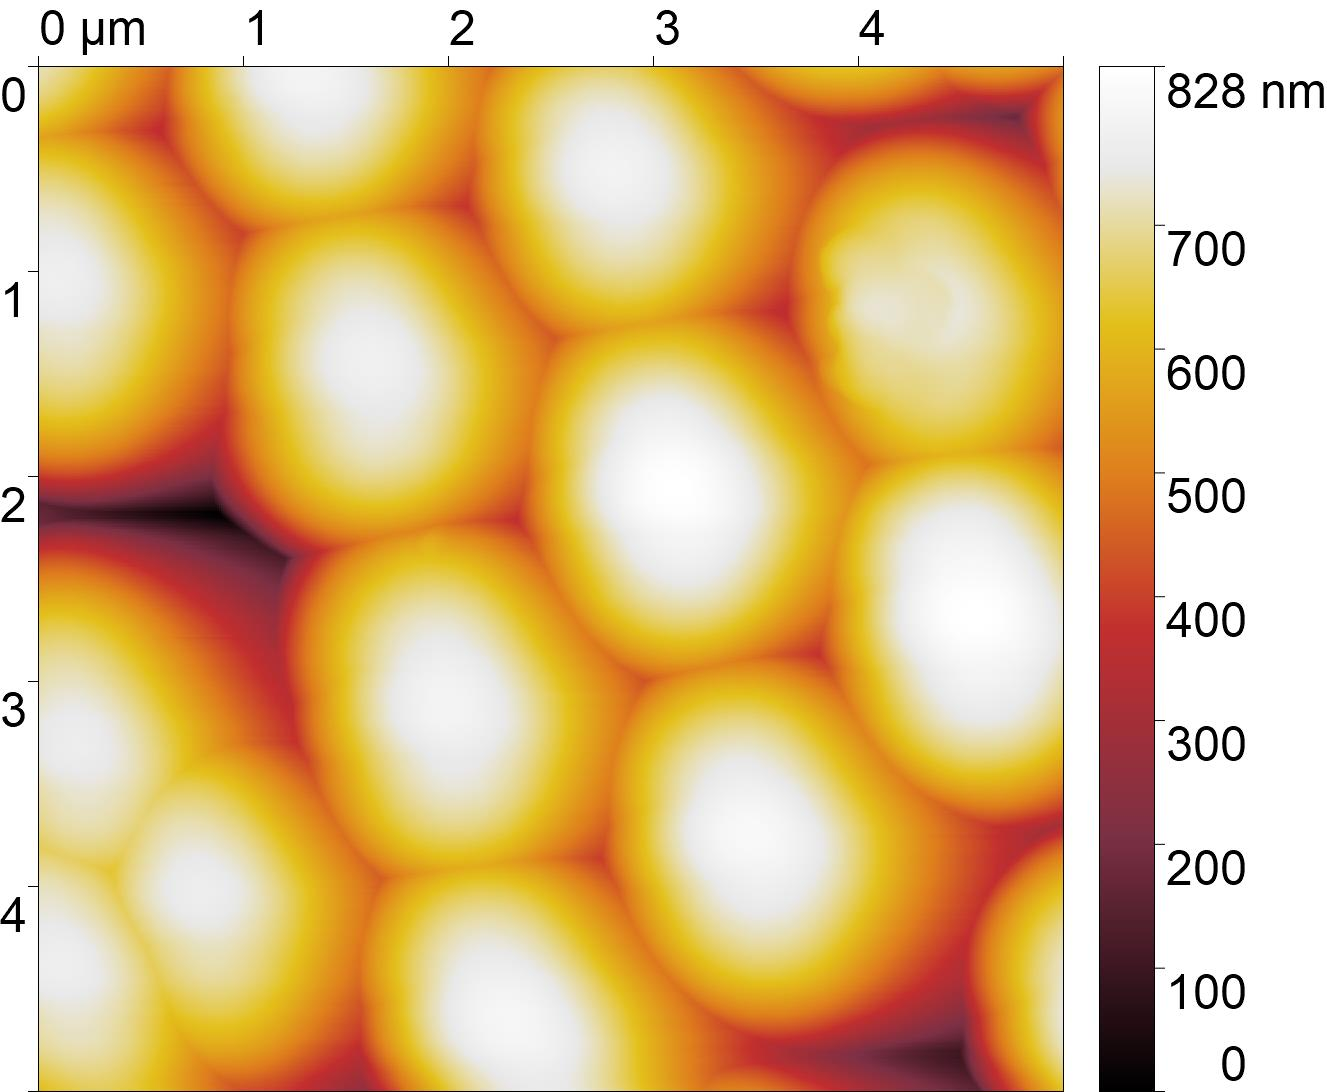
\includegraphics[width=90mm]{chapter3/5umareat2.jpg}
\end{center}
\caption{The observed surface of a silica sphere.}
\label{fig:SiliSph1}                 % Reference label to the figure.
\end{figure}

Initially, several scans were required in order to "zoom in" on an individual sphere. Due to the AFM's limit of 512 data points per line, the resolution of an individual sphere suffered unless it was the focus of the scanning frame. However, due to the drift in location due to pizeo error, attempting to suddenly zoom into a specific surface would dislocate the frame of reference from the intended area. As a result, an individual sphere was slowly zoomed in until it was the focus of the frame. This greatly reduced the range of images that could be taken and used.

Another feature of these sphere is their hexagon appearance under AFM. This is due to the tip's geometry, which limits the area it can reach, and therefore probe. As the geometry of the tip is pyramidal in shape and the true shape of the sphere is spherical, the areas that are unreachable by the probe are reported with a straight line and the height around the sphere are erroneously high. However, due to the intent of the procedure being focused on mapping the surface of a sphere, this does not affect the results as an area outside of this interference was chosen.



\begin{figure}[h]     %Insert a figure as soon as possible
        \begin{center}
          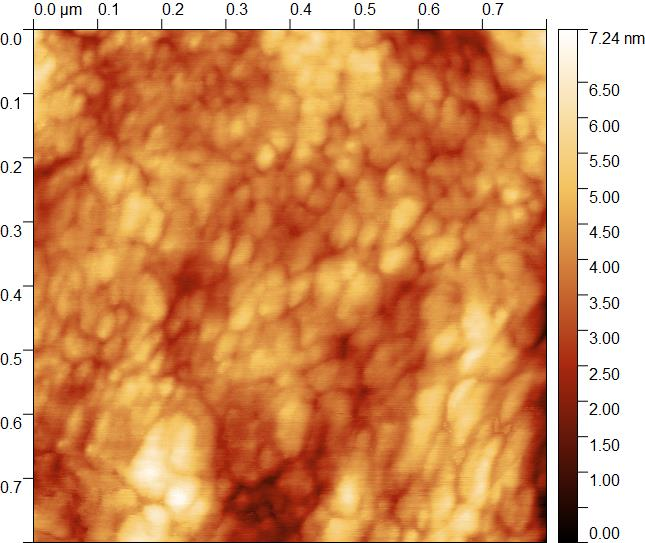
\includegraphics[width=100mm]{chapter3/Sphere3.jpg}
\end{center}
\caption{The flattened surface of a silica sphere.}
\label{fig:SiliSph2}                 % Reference label to the figure.
\end{figure}

The curvature inherent to the spherical geometry of silica beads presents a unique challenge for AFM analysis. Subsequent to imaging, any dataset inclinations or plane shifts were computationally rectified to ensure an accurate representation of the surface topology. This step was performed to remove any systematic tilt or distortion that could obscure the genuine surface features being studied. To isolate the surface characteristics accurately, advanced image processing techniques were employed. A 5th order polynomial fit was applied to \ref{fig:SiliSph1} in order to produce \ref{fig:SiliSph2}, effectively removing the curvature and normalizing the data to a flat plane. Further refinement was achieved by cropping the image, ensuring that only the relevant surface area remained within the data frame.

An AFM imaging of 3 1.5 $\mu$m silica spheres was performed, and spherical deconvolution was subsequently executed using Gwyddion software \cite{gwy}. From three functional sites across different spheres, an average RMS roughness of 0.65 nm was discerned, highlighting a notable difference in roughness compared to borosilicate glass. This suggests that silica spheres exhibit a higher degree of surface roughness.

\begin{figure}[h!!!!!]     %Insert a figure as soon as possible
        \begin{center}
          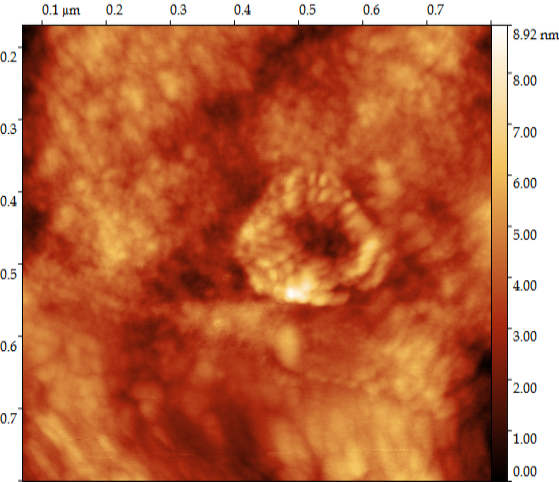
\includegraphics[width=100mm]{chapter3/Sili2.png}
\end{center}
\caption{The flattened surface of a silica sphere with a uniquely seen feature. The RMS roughness of this image was 0.72 nm, the highest one in the dataset.}
\label{fig:SiliSph3}                 % Reference label to the figure.
\end{figure}

The unique feature observed in \ref{fig:SiliSph3} could originate from various sources: a surface defect, an impurity, manufacturing-induced irregularities like bubbles or pits, or possibly artifacts related to the AFM process, such as tip convolution effects. Further investigative work is suggested to understand the adhesive interactions between silica particles and to determine if the central ``pit" seen in the images is a consequence of sonication used to disperse the silica spheres during the creation process. \cite{SilicaGrowth}

\newpage